\chapter{Types in C}
\label{ch:types}

\newcommand{\lecnum}{21}
%\newcommand{\lectitle}{Types in C}
\newcommand{\lecturer}{Frank Pfenning, Rob Simmons, Iliano Cervesato}

\chapterTAGS{c-numbers, casting, correctness, implementation-defined, other-types, undefined-behavior}
\maketitle

\begin{preamble}
\noindent
Previous lectures have emphasized the things we \emph{lost} by going to C:
\begin{itemize}
\item%
  Many operations that would safely cause an error in C0, like
  dereferencing \lstinline'NULL' or reading outside the bounds of an
  array, are \emph{undefined} in C --- we cannot predict or reason
  about what happens when we have undefined behaviors.
\item%
  It is not possible to capture or check the length of C arrays.
\item%
  In C, pointers and arrays are the same --- and we declare them like
  pointers, writing \lstinline'int *i'.
\item%
  The C0 types \lstinline'string', \lstinline'char*' and
  \lstinline'char[]' are all represented as pointers to
  \lstinline'char' in C.
\item%
  C is not garbage collected, so we have to explicitly say when we
  expect memory to be freed, which can easily lead to memory leaks.
\end{itemize}
In this lecture, we will endeavor to look on the bright side and
explore some of the new things that C gives us. But remember: with
great power comes great responsibility.  Today we will look at the
different ways that C represents numbers and the general, though
mostly implementation-defined, properties of these numbers that we
frequently count on.
\end{preamble}

\section{Numbers in C}
\label{sec:types:c_numbers}
\TAGS{c-numbers, undefined-behavior}

In addition to the undefined behavior resulting from bad memory access
(dereferencing a \lstinline'NULL' pointer or reading outside of an array),
there are other undefined behaviors in C. In particular:
\begin{itemize}
\item%
  Division by zero is undefined. (In C0, this always causes an exception.)
\item%
  Shifting left or right by negative numbers or by too-large a number is
  undefined. (In C0, this always causes an exception.)
\item%
  Arithmetic overflow for \emph{signed} types like \lstinline'int' is
  undefined. (In C0, this is defined as modular arithmetic.)
\end{itemize}

This has some strange effects. If \lstinline'x' and \lstinline'y' are signed
integers, then the expressions \lstinline'x < x+1' and \lstinline'x/y == x/y'
are either \lstinline'true' or undefined (due to signed arithmetic or
overflow, respectively).  So the compiler is allowed to pretend that
these expressions are just \lstinline'true' all the time. The compiler is
also allowed to behave the same way C0 does, returning \lstinline'false' in
the first case when \lstinline'x' is the maximum integer and raising an
exception in the second case when \lstinline'y' is 0. The compiler is also
free to check for signed integer overflow and division by zero and
start playing Rick Astley's ``Never Gonna Give You Up'' if either
occurs, though this last option is unlikely in practice.  Undefined
behavior is unpredictable --- it can and does change dramatically
between different computers, different compilers, and even different
versions of the same compiler.

The fact that signed integer overflow is undefined is particularly
annoying. A check like \lstinline'(x + 1 > x)', which was a perfectly
acceptable way to check that \lstinline'x' was not \lstinline'int_max()'
in C0, is now a check that the compiler is allowed to optimize to just
\lstinline'true', because the result of this expression, in C, is
either \lstinline'true' or undefined.

There are two ways of coping with signed integer overflow being
undefined. One option is to use \emph{unsigned} types, which are
required to obey the laws of modular arithmetic: \lstinline'unsigned int'
instead of \lstinline'int'.  As an example, consider a simple function to
compute Fibonacci numbers.  There are even faster ways of doing this,
but what we do here is to allocate an array on the stack, fill it with
successive Fibonacci numbers, and finally return the desired value at
the end.
\begin{lstlisting}[language=c, numbers=left]
unsigned int fib(unsigned int n) {
  unsigned int A[n+2];			/* stack-allocated array A */
  A[0] = 0;
  A[1] = 1;
  for (unsigned int i = 0; i <= n-2; i++)
    A[i+2] = A[i] + A[i+1];
  return A[n];  /* deallocates A just before actual return */
}
\end{lstlisting}

There's another solution, particular to the compiler, \lstinline'gcc',
that we usually use to compile C programs. This compiler (as well as
other modern C compilers like \lstinline'clang'), has a flag
\lstinline'-fwrapv'. When we compile with \lstinline'-fwrapv', then
the compiler promises it will treat overflow from addition and
multiplication as signed two's complement modular arithmetic, exactly
like C0 does.


\section{Implementation-defined Behavior}
\label{sec:types:implementation_defined}
\TAGS{c-numbers, implementation-defined, undefined-behavior}

In addition to \lstinline'int', which is a signed type, there are the
signed types \lstinline'short' and \lstinline'long', and
\lstinline'unsigned' versions of each of these types ---
\lstinline'short' is smaller than \lstinline'int' and \lstinline'long'
is bigger. The numeric type \lstinline'char' is smaller than
\lstinline'short' and always takes up one byte.  The maximum and
minimum values of these numeric types can be found in the standard
header file \lstinline'<limits.h>'.

C, annoyingly, does not define whether \lstinline'char' is signed or
unsigned. A \lstinline'signed char' is definitely signed, a
\lstinline'unsigned char' is unsigned. The type \lstinline'char' can
be either signed or unsigned --- this is \emph{implementation
  defined}.

It is often very difficult to say useful and precise things about the
C programming language, because many of the features of C that we have
to rely on in practice are not part of the C standard. Instead, they
are things that the C standard leaves up to the implementation ---
implementation defined behaviors. Implementation-defined behaviors
make it quite difficult to write code on one computer that will
compile and run on another computer, because the other compiler may
make completely different choices about implementation-defined
behaviors.

The first example we have seen is that, while a \lstinline'char' is
always exactly one byte, we don't know whether it is signed or
unsigned --- whether it can represent integer values in the range
$\lbrack -128,128)$ or integer values in the range $\lbrack 0,256)$. And it is even
worse, because a byte can be more than 8 bits! If you really want to
mean ``8 bits,'' you should say \emph{octet}.

In this class we are going to rely on a number of
implementation-defined behaviors. For example, you can always assume
that bytes are 8 bits on the computers we're using for this class in
this decade.  When it is important to \emph{not} rely on integer sizes
being implementation-defined, it is possible to use the types defined
in \lstinline'<stdint.h>', which defines signed and unsigned types of
specific sizes. In the systems that you are going to use for
programming, you can reasonably expect a common set of
implementation-defined behaviors: \lstinline'char' will be an 8-bit
integer (maybe signed, maybe unsigned) and so on.

\clearpage
\noindent
This chart describes how the \lstinline'<stdint.h>' types match up to
the standard C types in most modern C compilers:
\begin{center}
% \begin{tabular}{@{}ll@{\hspace{2em}}|@{\hspace{2em}}ll@{}}
%    \multicolumn{2}{c|@{\hspace{2em}}}{\bf Signed}
%  & \multicolumn{2}{c}{\bf Unsigned}
\begin{tabular}{ll|ll}
   \textbf{Signed}
&&&\textbf{Unsigned}
\\  C
 & \lstinline'stdint.h'
 & \lstinline'stdint.h'
 & C
\\ [1ex]
   \lstinline'signed' \lstinline'char'
 & \lstinline'int8_t'
 & \lstinline'uint8_t'
 & \lstinline'unsigned char'
\\ \lstinline'short'
 & \lstinline'int16_t'
 & \lstinline'uint16_t'
 & \lstinline'unsigned short'
\\ \lstinline'int'
 & \lstinline'int32_t'
 & \lstinline'uint32_t'
 & \lstinline'unsigned int'
\\ \lstinline'long'
 & \lstinline'int64_t'
 & \lstinline'uint64_t'
 & \lstinline'unsigned long'
\end{tabular}
\end{center}
However, please remember that we cannot count on this correspondence
behavior in \emph{all} C compilers!

There is another crucial numerical type: \lstinline'size_t', is the
type used represent memory sizes and array indices. The
\lstinline'sizeof(ty)' operation in C actually returns just the size
of a type in bytes, so \lstinline'malloc' and \lstinline'xmalloc'
actually take one argument of type \lstinline'size_t' and
\lstinline'calloc' and \lstinline'xcalloc' take two arguments of type
\lstinline'size_t'. As we approach the third decade of the 21st
century, we're increasingly using 64-bit systems and not dealing with
32-bit systems anymore. On 32-bit systems, \lstinline'size_t' is
usually 4-byte, 32-bit unsigned integer. We now usually expect
\lstinline'size_t' to be a 64-bit, 8-byte unsigned integer.

%% still used to finding both 32-bit and 64-bit machines and programs;
%% \lstinline'size_t' will usually be the same as \lstinline'uint32_t'
%% in a 32-bit system and the same as \lstinline'uint64_t' in a 64-bit
%% system.  The same goes for \lstinline'uintptr_t', an integer type
%% used to represent pointers. Everything in C has an address, every
%% address can be turned into a pointer with the address-of operation,
%% and every address is ultimately representable as a number. To make
%% sense of what it means to store a pointer in a integer type, we're
%% going to need to introduce a new topic, \emph{casting}.

\section{Casting Between Numeric Types}
\label{sec:types:casting}
\TAGS{casting, c-numbers, implementation-defined}

Now that we've introduced a bunch of different integer types, we need
to see how to work with multiple integer types in the same program.

Imagine we have the hexadecimal value \lstinline'0xF0' --- represented
as a sequence of bits as \lstinline'11110000' --- stored in an
unsigned \lstinline'char', and we want to turn that value into an
\lstinline'int'.  (This is a problem you will actually encounter later
in this semester.) We can \emph{cast} this character value to an
integer value by writing \lstinline'(int)e'.
\begin{lstlisting}[language=c]
  unsigned char c = 0xF0;
  int i = (int)c;
\end{lstlisting}
However, what will the value of this integer be? You can run this code
and find out on your own, but the important thing to realize is that it's
not clear, because there are two different stories we can tell.

In the first story, we start by transforming the unsigned
\lstinline'char' into an unsigned \lstinline'int'. When we cast from a
small unsigned quantity to a large unsigned quantity, we can be sure
that the \emph{value} will be preserved. Because the bits
\lstinline'11110000' are understood as the unsigned integer 240, the
unsigned \lstinline'int' will also be 240, written in hexadecimal as
\lstinline'0x000000F0'. Then, when we cast from an unsigned
\lstinline'int' to a signed \lstinline'int', we can expect the bits to
remain the same (though this is really implementation defined), and
because the interpretation of signed integers is two's-complement
(also implementation defined) the final value will be 240.

In the second story, we first transform the unsigned \lstinline'char'
into a signed \lstinline'char'. Again, the implementation-defined
behavior we expect is that we will interpret the result as an 8-bit
signed two's-complement quantity, meaning that \lstinline'0xF0' is
understood as $-16$.  Then, when we cast from the small signed
quantity (\lstinline'signed char') to a large signed quantity
(\lstinline'int'), we know the quantity $-16$ will be preserved,
meaning that we will end up with a signed integer written in
hexadecimal as \lstinline'0xFFFFFFF0'. In order to preserve the value
as we go from a small to a large signed quantity, all we have to do is
use \emph{sign extension} --- copy the high-order bit into all the new
spaces.
\begin{center}
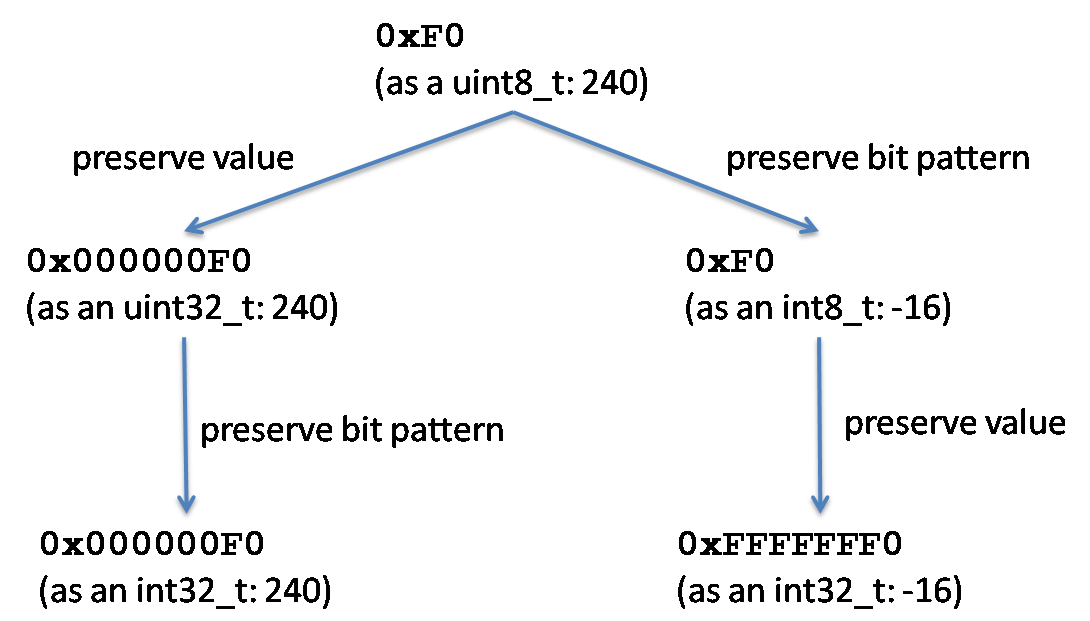
\includegraphics[width=0.8\textwidth]{img/cast.png}
\end{center}

The order in which we do these two steps matters! Therefore, if we
want to be clear about what result we want, we should cast in smaller
steps to be explicit about how we want our casts to work:
\begin{lstlisting}[language=c]
  unsigned char c = 0xF0;
  int i1 = (int)(unsigned int) c;
  int i2 = (int)(signed char) c;
  assert(i1 == 240);
  assert(i2 == -16);
\end{lstlisting}
The C standard does define which of these two things will happen when
you cast directly from \lstinline'unsigned char' to
\lstinline'int'. However, for the purposes of this class, where we're
trying to teach you enough C to write clear and correct programs, it's worth
obeying the following rules:
\begin{itemize}
\item%
  Never cast between signed and unsigned types of \emph{different
    sizes}.  Only cast between signed and unsigned types with the same
  size (implementation defined to preserve bits) and between small and
  large types that are either both signed or both unsigned.
\item%
  When you cast from a large signed (or unsigned) type to a small
  signed (or unsigned) type, make sure that the type you're casting to
  can represent the number. (So, for instance, you can cast the
  \lstinline'int' 17 to an signed \lstinline'char', but don't cast the
  \lstinline'int' 1000 to a signed \lstinline'char', because a signed
  \lstinline'char' can only represent numbers between -128 and 127,
  inclusive.)
\item%
  When you add, subtract, multiply, divide, compare, or do bitwise
  operations involving multiple variables, it's best to make sure that
  all the numbers you're working with have the same size and same
  signedness. One important ``gotcha'' here: if you just write the
  number \lstinline'4', it's treated as an \lstinline'int' by default,
  so writing
\begin{lstlisting}[language=c]
int64_t i = 1 << 40;
\end{lstlisting}

will actually be undefined behavior, because \lstinline'1' is
(implementation-defined to be) a 32-bit quantity that can only be
shifted by numbers between 0 and 31, inclusive. The fix, in this
situation, is to write:
\begin{lstlisting}[language=c]
int64_t i = 1;
i = i << 40;
\end{lstlisting}
\end{itemize}


\section{Other Types In C}
\label{sec:types:enum_union_float_double}
\TAGS{correctness, other-types}

C introduces a number of other types as well that we didn't have in
C0.  In particular, many C programs use \lstinline'enum' types,
\lstinline'union' types, and the floating point types,
\lstinline'float' and \lstinline'double', which are used to represent
fractional numbers like \lstinline'0.25'. You'll learn much more about
these other C types in later courses, like 15-213, but here are the
basics.

\subsection{Floating Point}
\label{sec:types:floats}

The C type \lstinline'float' allows writing numbers such as $0.1$ and
$3.14159265$ as well as $2.2035 \times 10^{-27}$ (entered as
\lstinline'2.2035E-27') that have a fractional component.  It also
allows writing very large numbers such as $10^{20}$ that are not
representable as \lstinline'int''s.  \lstinline'float' provides
\emph{floating point numbers} as a way to work with numbers other than
integers, in particular (some) rational numbers.  The size of a
\lstinline'float' is implementation-defined, although it is typically
32 bits in modern computers.  Those 32 bits is all that is available
to represent floating point numbers --- the same as \lstinline'int''s
--- but the range these numbers are drawn from is much wider:
$10^{20}$ and $-10^{20}$ can both be entered as \lstinline'float''s
although much larger than \lstinline'INT_MAX' and much smaller than
\lstinline'INT_MIN' respectively, and so is $10^{-20}$.  What gives?
\emph{Precision}.

The following simple program divides $10^{20}$ by $10^{10}$ and
multiplies the outcome by $10^{10}$.  We expect the final result to be
$10^{20}$.
\begin{lstlisting}[language=c]
void main() {
  float x = 10E20;
  float y = 10E10;
  printf("%f\n", (x/y)*y);
}
\end{lstlisting}
Instead, it outputs \lstinline'999999949672133165056.000000' ---
almost $10^{20}$ but not quite.

C offers another type for floating point numbers, \lstinline'double',
which stands for \emph{double precision} (its size is again
implementation-defined and typically 64 bits in current hardware).
The above example works as expected if we replace \lstinline'float'
with \lstinline'double', but a similar example which uses bigger
numbers will suffer from the same problem: double precision is not
infinite precision.

Precision loss during calculations, as just witnessed, makes it all
but impossible to reason about programs that use floating point
numbers.  This is why \lstinline'float' was left out of C0.

Here's another example:
\begin{lstlisting}[language=c]
  for (float res = 0.0; res != 5.0; res += 0.1) {
    printf("res = %f\n", res);
  }
  printf("Done!\n");
\end{lstlisting}

We would expect the loop to run some 50 times, then exit and print
\lstinline'Done!'.  Instead, it keeps running, printing ever larger
values of \lstinline'res':
\begin{lstlisting}[language={[coin]C}]
# a.out
res = 0.000000
res = 0.100000
res = 0.200000
                ... [elided]
res = 2.600000
res = 2.700000
res = 2.799999
res = 2.899999
                ... [elided]
res = 4.999998
res = 5.099998
                ... [elided]
res = 8.799997
res = 8.899998
                ... [elided]
\end{lstlisting}
After a few iterations, the value of \lstinline'res' starts deviating
from what we expect --- a single decimal digit followed by zeros ---
and eventually passes 5.0 because it is never equal to that value.
How is this possible with simple numbers like \lstinline'0.1' and
\lstinline'5.0'?  These numbers, as we entered them in the program,
are in decimal.  The compiler automatically converts them into binary
using a very similar procedure as what we saw for integers.  Take
\lstinline'0.1'.  We obtain the fractional part (or \emph{mantissa})
by repeatedly multiplying this number by 2 and harvesting the digit to
the left of the decimal point until we get $0.0$:
$$
\begin{array}{l@{\;\;\times\;\; 2 \;\;\;=\;\;\;}l@{\;\;\;\text{yields}\;\;\;}ll}
   0.1 & \mathbf{0}.2  & 0
\\ 0.2 & \mathbf{0}.4  & 0
\\ 0.4 & \mathbf{0}.8  & 0
\\ 0.8 & \mathbf{1}.6  & 1 & \text{subtract 1}
\\ 0.6 & \mathbf{1}.2  & 1 & \text{subtract 1}
\\ 0.2 & \mathbf{0}.4  & 0
\end{array}
$$
and so on.  Notice that we have seen $0.2$ before, and therefore the process
repeats \ldots infinitely.  The number $0.0$, at which point we would
stop, never emerges.  What is happening is that, while $0.1$ has a
finite mantissa in decimal (just one digit after the decimal point),
it has an infinite mantissa in binary: $0.1_{10}$ is a periodic number
in binary --- $0.0\overline{0011}_2$.  This means that a precise
representation as a binary mantissa cannot be achieved with any fixed
number of bits.  Thus the value of \lstinline'x' above is an
approximation of $0.1$ rather than exactly this number.  It is printed
out as \lstinline'0.100000' thanks to rounding but, as we keep on
adding it to itself with ``\lstinline'res += x''' errors accumulate
since we are working with an approximation of $0.1$, and these errors
eventually manifest when printing \lstinline'res'.


\subsection{Union and enum types}
\label{sec:types:enum_union}

As a way to introduce some additional features of C, consider a type
of trees that carry their data in their leaves rather than in the
inner nodes (we call them \emph{leafy trees} and they are at the basis
of data structures used in the implementation of database management
systems and in other areas of computer science).  A leafy tree can be
a leaf carrying a value, it can be an inner node with no value but
left and right children, it can also be empty which contains neither a
value nor children.

Based on the fragment of C we know so far, we would use the following
type to define the nodes of a leafy tree with integer values:
\begin{lstlisting}[language=c]
typedef struct ltree leafytree;
struct ltree {
  int nodetype;
  int data;
  leafytree *left;
  leafytree *right;
};
\end{lstlisting}
We use the field \lstinline'nodetype' to distinguish the type of the
node (a leaf, an inner node, or empty\footnote{An alternative is to
  represent the empty leafy tree as \lstinline'NULL'.  We refrain from
  doing so to make this example more interesting.}).  This
representation wastes memory: inner nodes do not make use of the
\lstinline'data' field, while \lstinline'left' and \lstinline'right'
are meaningless for a leaf, and furthermore all 3 for go unused for
the empty tree.  As we will see shortly, C provides a mechanism to
mitigate this problem.

Before examining it, let's go back to \lstinline'nodetype': we need to
pick three values to denote the three types of nodes, but we use the
space for an entire \lstinline'int' for them --- more waste.  C
provides \emph{enum types} as a way to shield the programmer both from
picking constants whose values are to all effects irrelevant as long as
they are distinct and in deciding exactly how much memory to allocate.
In our example, this is done through the declaration
\begin{lstlisting}[language=c]
enum nodetype { INNER, LEAF, EMPTY };
\end{lstlisting}
From now on, we can use the mnemonic constants \lstinline'INNER',
\lstinline'LEAF' and \lstinline'EMPTY' as type indicators for our
various nodes.

\emph{Union types} provide a way to view an area of memory as having
more than one type.  Here, the memory associated with a node needs to
be viewed either as an \lstinline'int' (for leaves) or as a pair of
pointers (for inner nodes).  We can do so using the following
declarations:
\begin{lstlisting}[language=c]
typedef struct ltree leafytree;
struct innernode {        // type of an inner node
  leafytree *left;
  leafytree *right;
};
union nodecontent {       // contents of a non-empty node:
  int data;               // EITHER an int
  struct innernode node;  //     OR and inner node
};
struct ltree {
  enum nodetype type;
  union nodecontent content;
};
\end{lstlisting}
Here, \lstinline'struct innernode' packages the two pointers needed
for inner nodes.  The type \lstinline'union nodecontent' can contain
either the integer \lstinline'data' or the value \lstinline'node' of
type \lstinline'struct innernode' --- but not both.  The compiler will
decide how to organize the memory for this union type (on modern
hardware, probably 16 byte viewed either as two 8-byte pointers or a
4-byte \lstinline'int' and 12 unused bytes).  Lastly, the definition of
\lstinline'struct ltree' contains the field \lstinline'type' of enum
type \lstinline'enum nodetype' defined earlier, and the field
\lstinline'content' of union type \lstinline'union nodecontent'.

% The definition of \lstinline'struct ltree' contains the field
% \lstinline'type' of enum type \lstinline'enum nodetype' defined
% earlier, and a union type that makes available either the field
% \lstinline'data' or the \lstinline'node' field --- but not both.
% The compiler will decide how to organize the memory for this union
% type (on modern hardware, probably 16 byte viewed either as two
% 8-byte pointers or a 4-byte \lstinline'int' and 12 unused bytes).

We define an actual leafy tree as in the following example:
\begin{lstlisting}[language=c]
  leafytree *T = malloc(sizeof(leafytree));
  T->type = INNER;
  T->content.node.left = malloc(sizeof(leafytree));
  T->content.node.left->type = EMPTY;
  T->content.node.right = malloc(sizeof(leafytree));
  T->content.node.right->type = LEAF;
  T->content.node.right->content.data = 42;
\end{lstlisting}
Note that the \lstinline'type' fields are assigned the symbolic
constants in our enum type.  Notice also that we access the
alternatives of a union type using the dot notation, as in
\lstinline'T->content.node.left'.  It is left to the discipline of the
programmer to use these fields consistently, for instance not to
access the \lstinline'data' component of an \lstinline'INNER' node.

Before we are done with this example, let's introduce a useful
construct of C, especially in the presence of enum type definitions:
the \lstinline'switch' statement.  The following recursive function
adds all the values stored in (the leaves of) a leafy tree:

\begin{lstlisting}[language=c]
int add_tree(leafytree *T) {
  int n = 0;
  switch (T->type) {
  case INNER:
    n += add_tree(T->content.node.left);
    n += add_tree(T->content.node.right);
    break;

  case LEAF:
    n = T->content.data;
    break;

  default:
    n = 0;
  }

  return n;
}
\end{lstlisting}
The construct \lstinline'switch' discriminates on the value of
\lstinline'T->type', jumping to the appropriate \lstinline'case'
block.  If a \lstinline'case' block is not given for a value, the
execution proceeds to the \lstinline'default' block which is always
the last (although a programmer may decide to omit it).  Each block
except the last typically needs to end with a \lstinline'break'
statement, otherwise the execution will proceed with the next block
rather than exiting the \lstinline'switch' statement.
